

%--------------------------------------------------------
\subsubsection*{The power law rheology}
\index{general}{Power Law Rheology}
\index{general}{Generalised Power Law Rheology}

In what follows the viscosity 
is assumed to be of the power law type, i.e.
\[
\eta(\dot{\bm \varepsilon}) = \beta  \dot{\varepsilon}_e^{\frac1n-1}
\]
where $\beta$ is a scalar, $n$ is a small number (but not 
necessarily an integer) and
$\dot{\varepsilon}_e$ is the effective strain rate defined in Eq.~\eqref{eq:tauepse},
i.e.
\[
\dot\varepsilon_e = \sqrt{ \frac{1}{2}(\dot\varepsilon_{xx}^2 + \dot\varepsilon_{yy}^2 ) 
+ \dot\varepsilon_{xy}^2}
\]
We will also consider the generalised power-law rheology:
\[
\eta_{\dot\gamma}(\dot{\bm \varepsilon})  = \beta  ( \dot{\varepsilon}_e^2 + \dot\gamma^2)^{\frac{1-n}{2n}}
\]
This formulation has the advantage that viscosity does not become infinite 
when the strain rate becomes zero.
Finally, to simplify notations we define $\alpha=\frac1n-1$ so that 
\[
\boxed{
\eta_{\dot\gamma}(\dot{\bm \varepsilon})  = \beta  ( \dot{\varepsilon}_e^2 + \dot\gamma^2)^{\alpha/2}
}
\qquad
\text{or simply}
\qquad
\boxed{
\eta(\dot{\bm \varepsilon})  = \beta  \dot{\varepsilon}_e^\alpha
}
\]




 

%--------------------------------------------------------------------
\subsubsection*{Newton-Raphson method for single-valued functions}

In numerical analysis, the Newton's method (also Newton-Raphson method) 
is an iterative root-finding algorithm.
The most basic version for a function $f(x)$ is as follows\footnote{\url{https://en.wikipedia.org/wiki/Newtons_method}}:
\[
x^{k+1} = x^k - \frac{f(x^k)}{f'(x^k)}
\]
where we assume that the derivative $f'$ exists and we start the iterations 
with a guess $x_0$.
If the function satisfies sufficient assumptions and the initial guess is close
to the real solution then the method converges to the root. 
Note that if a stationary point of the function is encountered, i.e. 
the derivative is zero, then the method will terminate due to division by zero. 

%--------------------------------------------------------------------
\subsubsection*{Newton-Raphson method for systems of equations}
Let us consider the following system of $N$ equations. 
\[
{\bm A} \cdot \vec{X} = \vec{b}
\]
Solving this system is equivalent to finding the root of 
\[
\vec{R}(\vec{X}) =  {\bm A} \cdot \vec{X} - \vec{b}
\]
i.e. finding the zeroes of the continuously differentiable function $\vec{R}: \R^N \rightarrow \R^N$. 
In this case, the Newton algorithm is written as a function of the $N\times N$ Jacobian 
matrix ${\bm J}_R$:
\begin{equation}
\vec{X}^{k+1} = \vec{X}^k - {\bm J}_R^{-1}(\vec{X}^k) \cdot {\vec R}(\vec{X}^k)
\end{equation}
or,
\begin{equation}
{\bm J}_R (\vec{X}^k) \cdot( \vec{X}^{k+1} - \vec{X}^k  )   = - \vec{R}(\vec{X}^k)
\label{eq:f87newt}
\end{equation}
where the Jacobian matrix is defined as follows\footnote{\url{https://en.wikipedia.org/wiki/Jacobian_matrix_and_determinant}}:
\[
{\bm J}_R = 
\left(
\begin{array}{ccc}
\frac{\partial R_1}{\partial X_1} & \dots & \frac{\partial R_1}{\partial X_N} \\
\vdots & \ddots & \vdots \\ 
\frac{\partial R_N}{\partial X_1} & \dots & \frac{\partial R_N}{\partial X_N} 
\end{array}
\right)
\]



%----------------------------------------------------------------
\subsubsection*{The super simple / no questions asked approach}


We have to solve 
\[
{\bm A}(\vec{X}) \cdot \vec{\cal X} = \vec{b}
\]
where the matrix ${\bm A}(\vec{\cal X})$ comes from the discretization of the incompressible
Stokes equations and the vector $\vec{b}$ corresponds to body forces, surface forces and 
boundary conditions. We assume here for simplicity that $\vec{b}$
is independent of the vector of unknowns $\vec{X}$, which is made of
$\vec{\cal V}$ and $\vec{\cal P}$. The dependence of ${\bm A}$ on $\vec{\cal X}$ 
comes from the dependence of the viscosity on strain rate (and therefore velocity)
and pressure (although in this particular case of the power law rheology pressure does 
not enter the equations). 

The matrix ${\bm A}(\vec{\cal X})$ has the following structure:
\begin{equation}
{\bm A}(\vec{\cal X}) = 
\left(
\begin{array}{cc}
\K(\vec{\cal X}) & \G  \\
\G^T & 0 
\end{array}
\right)
\end{equation} 
and the discretised Stokes system is then
\begin{equation}
\left(
\begin{array}{cc}
\K(\vec{\cal V}) & \G  \\
\G^T & 0 
\end{array}
\right)
\cdot
\left(
\begin{array}{cc}
\vec{\cal V} \\
\vec{\cal P} \\
\end{array}
\right)
=
\left(
\begin{array}{cc}
\vec{f} \\ \vec{h}
\end{array}
\right)
\end{equation}
The discrete residual is defined by 
\begin{eqnarray}
\vec{\cal R}(\vec{\cal X}) 
&=& {\bm A}(\vec{\cal X})\cdot \vec{\cal X} - \vec{b} \label{eq:f87_res} \\
&=& 
\left(
\begin{array}{c}
\K(\vec{\cal V}) \cdot \vec{\cal V} + \G \cdot \vec{\cal P} - \vec{f} \\
\G^T \cdot \vec{\cal V} - \vec{h}
\end{array}
\right) \\
&=&
\left(
\begin{array}{cc}
\vec{R}_{\cal V} \\
\vec{R}_{\cal P} 
\end{array}
\right)
\end{eqnarray}




\paragraph{Standard Picard iterations} are as follows:
\begin{equation}
\boxed{
{\bm A}(\vec{\cal X}^k) \cdot \vec{\cal X}^{k+1} = \vec{b} \label{eq:f87_picard}
}
\end{equation}

\paragraph{Defect Picard iterations}
We can use Eq.~\eqref{eq:f87_res} to write 
$\vec{b} = {\bm A}(\vec{\cal X}^k)\cdot \vec{\cal X}^k  -\vec{R}(\vec{\cal X}^k)$
and then replace $\vec{b}$ in Eq.~\eqref{eq:f87_picard}:
\begin{equation}
{\bm A}(\vec{\cal X}^k) \cdot \vec{\cal X}^{k+1} 
= {\bm A}(\vec{\cal X}^k)\cdot \vec{\cal X}^k -\vec{R}(\vec{\cal X}^k)
\end{equation}
and finally, defining $\delta\vec{\cal X}^{k} = \vec{\cal X}^{k+1} -\vec{\cal X}^{k}$, 
we can write 
\[
\boxed{
{\bm A}(\vec{X}^k) \cdot \delta \vec{X}^{k} = -\vec{R}(\vec{X}^k)
}
\]
This approach must be supplemented with 
\[
\vec{\cal X}^{k+1} = \vec{\cal X}^k + \delta \vec{\cal X}^{k} 
\]



\paragraph{Newton iterations}
We start from 
\[
\vec{\cal R}(\vec{\cal X}) = {\bm A}(\vec{\cal X})\cdot \vec{\cal X} - \vec{b} 
\]
and apply the methodology of Eq.~\eqref{eq:f87newt} 
and a Newton iteration then consists of solving 
for $\delta \vec{\cal X}^{k}$ the following linear system  
\[
\boxed{
{\bm J}_R(\vec{\cal X}^k) \cdot \delta \vec{\cal X}^{k} = -\vec{R}(\vec{\cal X}^k)
}
\]
and updating $\vec{\cal X}^k$:
\begin{equation}
\vec{\cal X}^{k+1} = \vec{\cal X}^k + \delta \vec{\cal X}^{k} 
\label{eq:f87updt}
\end{equation}
Note that we recover the defect correction Picard when setting ${\bm J}_R \rightarrow {\bm A}$.
Also, the update of Eq.~\eqref{eq:f87updt} can be rewritten
\[
\vec{\cal X}^{k+1} = \vec{\cal X}^k + \upalpha^k \delta \vec{\cal X}^{k} 
\]
where $\upalpha$ is a step length parameter that can be determined, for example, using
a line search.


Deriving the exact expression for ${\bm J}_R$ is actually where the difficulty really lies.
From the structure of ${\bm A}$, we expect the Jacobian matrix to take the form
\[
{\bm J}_R = 
\left(
\begin{array}{cc}
\J_{vv} & \J_{vp}  \\
\J_{pv} & 0 
\end{array}
\right)
\] 

The term $\J_{vv}$ corresponds to the derivative of
$\vec{R}_{\cal V}= \K(\vec{\cal V}) \cdot \vec{\cal V} + \G \cdot \vec{\cal P} - \vec{f}$
with respect to $\vec{\cal V}$
For a power law rheology, it can be written\footnote{Skipping a lot of steps for now}
\[
\J_{vv}(\vec{\cal X}^k) = \K_0(\vec{\cal V}^k)+\K_1(\vec{\cal V}^k)
\]
where $\K_0$ is the standard matrix obtained from 
\begin{eqnarray}
\K_0 &=& \int_\Omega \eta(\dot{\bm \varepsilon}^k) {\bm B}^T \cdot {\bm C} \cdot  {\bm B} dV \\
\K_1 &=& 
\end{eqnarray}


The term $\J_{vp}$ corresponds to the derivative of 
$\vec{R}_{\cal V}= \K(\vec{\cal V}) \cdot \vec{\cal V} + \G \cdot \vec{\cal P} - \vec{f}$ 
with respect to $\vec{\cal P}$. Since the viscosity does not depend on pressure, 
then we have $\J_{vp}=\G$.
Likewise $\J_{pv}$ corresponds to the derivative of
$\vec{R}_{\cal V}= \G^T \cdot \vec{\cal V} -\vec{h}$  with respect to $\vec{\cal V}$
which yields $\J_{vp}=\G^T$.
Finally 
\[
{\bm J}_R = 
\left(
\begin{array}{cc}
\K_0(\vec{\cal V}) + \K_1(\vec{\cal V}) & \G  \\
\G^T & 0 
\end{array}
\right)
\] 
This justifies why we have chosen a power law rheology to start with the implementation of 
the Newton-Raphson method: the modifications to the FE matrix are small and limited 
to the viscous block and the rhs is simply the previous residual. 
 



%---------------------------------------------
\subsubsection*{Implementation details}

The code is a 'standard' $Q_2 \times Q_1$ element code which solves 
a few nonlinear problems, some of which having analytical solutions. 

It is established that the Newton method converges only if the initial guess is 'close enough'
to the real solution. It is then customary of carrying out a few Picard iterations 
before switching over to the Newton method. 
This is why we define the parameter $\theta\in[0,1]$ in the code such that 
\[
\J_{vv} = \K_0(\vec{\cal V})+\theta \K_1(\vec{\cal V})
\]
Indeed, if $\theta=0$ we recover the defect correction Picard method and
if $\theta=1$ we recover the standard Newton method. 
Moreover, the parameter $\theta$ can be adapted according to the norm of 
the residual, for example by choosing 
\[
\theta = 1 - \frac{||\vec{R}^k||}{||\vec{R}^1||}
\]
where $\vec{R}^1$ is the residual at the 1st iteration and 
as $||\vec{R}^k||$ becomes small, $\theta \rightarrow 1$.
This then ensures a smooth transition between both methods.

Concerning the defect Picard method, two main modifications 
are needed: build a different rhs, and adapt the boundary conditions. 
The (elemental) rhs is split across two arrays {\codefont f\_el} and {\codefont h\_el}.
In a standard code $f_el$ receives the contribution of the buoyancy forces at 
each quadrature point:
\begin{lstlisting}
for i in range(0,mV):
    f_el[ndofV*i+0]+=NNNV[i]*jcob*weightq*gx(xq,yq)*rho
    f_el[ndofV*i+1]+=NNNV[i]*jcob*weightq*gy(xq,yq)*rho
\end{lstlisting}
This is in fact the $\vec{b}$ term of Eq.\eqref{}. 
Also the array {\codefont h\_el} is zero before boundary conditions are
applied so there is no direct contribution to it inside the loop over 
quadrature points.

For each element we store the velocity and pressure field in dedicated arrays
{\codefont V\_el} and {\codefont p\_el}:

\begin{lstlisting}
V_el=np.zeros((mV*ndofV),dtype=np.float64)
P_el=np.zeros((mP*ndofP),dtype=np.float64)

for i in range(0,mV):
    V_el[2*i+0]=solution[2*iconV[i,iel]+0]
    V_el[2*i+1]=solution[2*iconV[i,iel]+1]

for i in range(0,mP):
    P_el[i]=p[iconP[i,iel]]
\end{lstlisting}
and we then proceed to add the necessary terms to both {\codefont f\_el} and {\codefont h\_el}:
\begin{lstlisting}
f_el-=K_el0.dot(V_el)+G_el.dot(P_el) 
h_el-=G_el.T.dot(V_el)               
\end{lstlisting}

The second modification concerns the boundary conditions. 
As per usual in our codes, there is an array {\codefont bc\_val} 
which contains the prescribed value of the boundary condition.
It is then necessary to transfer it to the global solution vector 
before iterations are carried out:
\begin{lstlisting}
solution[0:NfemV]=bc_val[0:NfemV]
\end{lstlisting}
Since the unknowns of the system are successive corrections on the 
velocity and pressure, we therefore need to start with the known 
values in the solution vector. Further down, when we apply boundary conditions, 
we must then apply zero, so that the correction is zero where 
boundary conditions are applied in the domain.  



%--------------------------------------------------------------------------
\subsubsection*{Experiment 0 - the linear (regularised) lid driven cavity}

The domain is a unit square. Free slip boundary conditions are prescribed on the 
left, right and bottom boundaries, while $\vec\upnu=(x(1-x),0$ is prescribed on the 
top. There are no buoyancy forces and the viscosity is set to 1. Although 
not necessary, the pressure is normalised so as to have a zero volume average. 
This is a linear problem and a single Stokes solve returns the solution. Any further 
iteration should then not alter this solution. 
Concretely, we expect that from the 2nd iteration the solution of the sytem $\delta {\cal X}$ 
is zero (down to machine precision).

\begin{center}
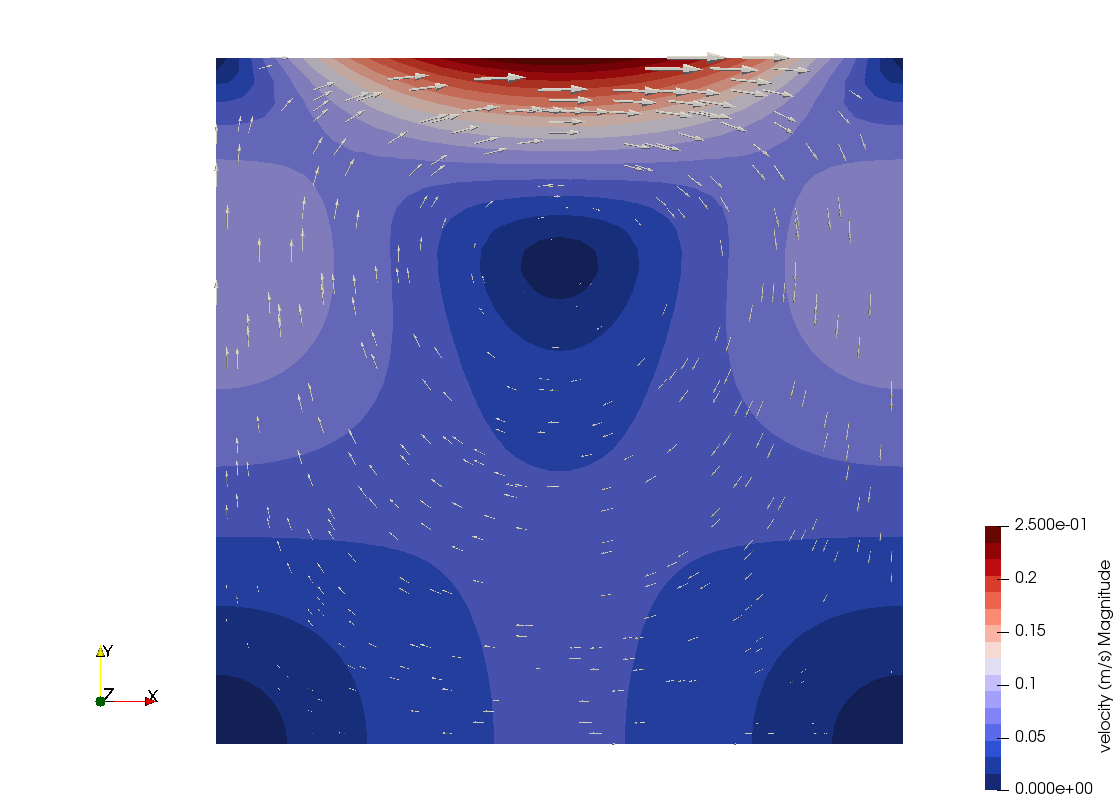
\includegraphics[width=5.5cm]{python_codes/fieldstone_87/results/experiment_00/vel}
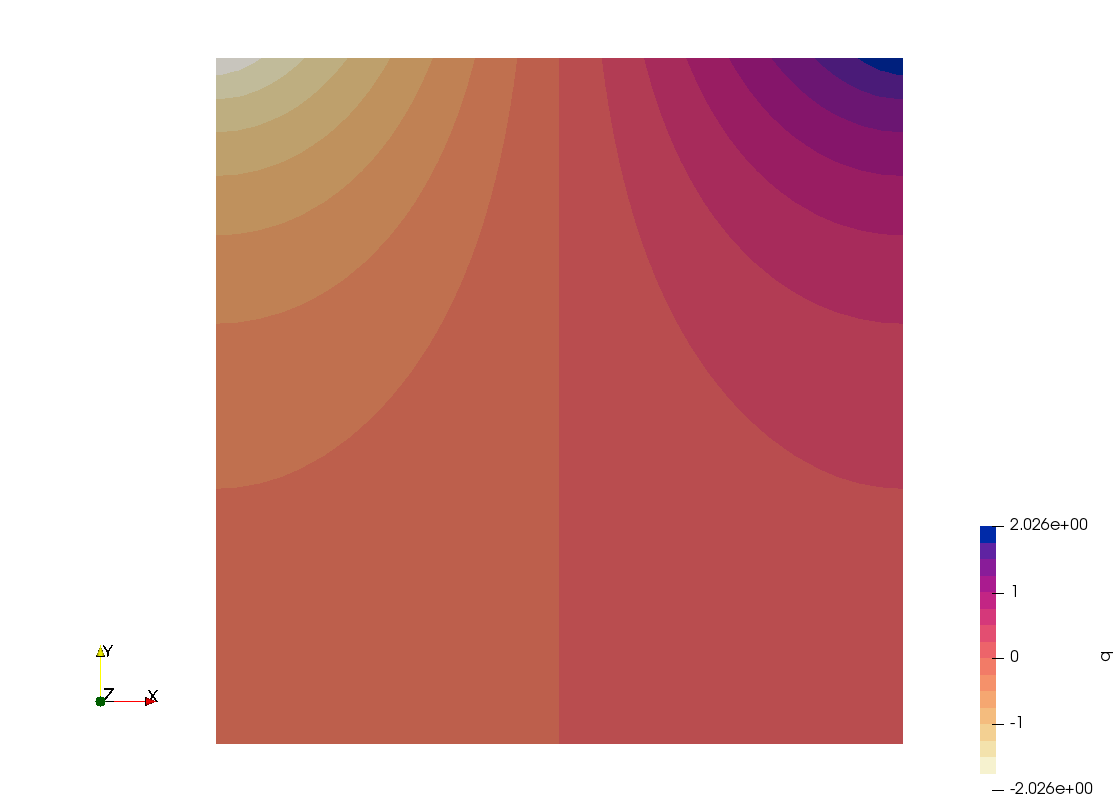
\includegraphics[width=5.5cm]{python_codes/fieldstone_87/results/experiment_00/p}
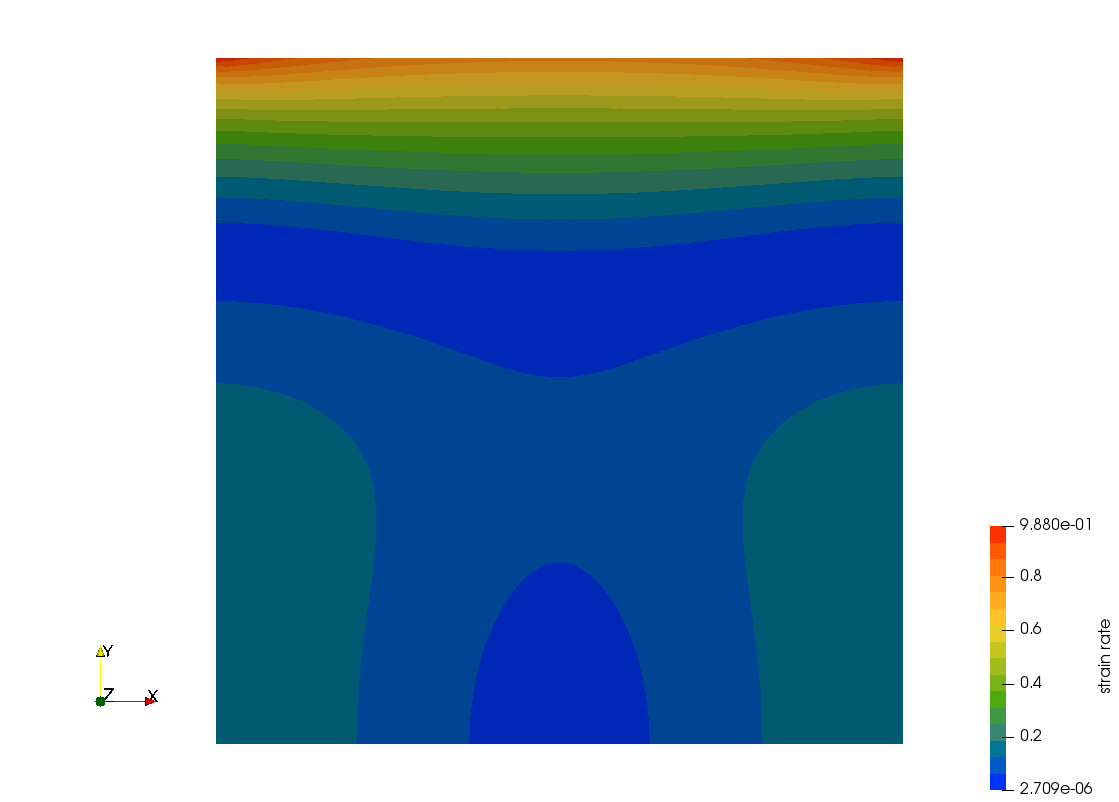
\includegraphics[width=5.5cm]{python_codes/fieldstone_87/results/experiment_00/sr}\\
{\captionfont Solution as obtained on a $32\times 32$ grid.}
\end{center}

Four defect Picard iterations are carried out and the solution fields for 
each iteration are shown here under:  

\begin{center}
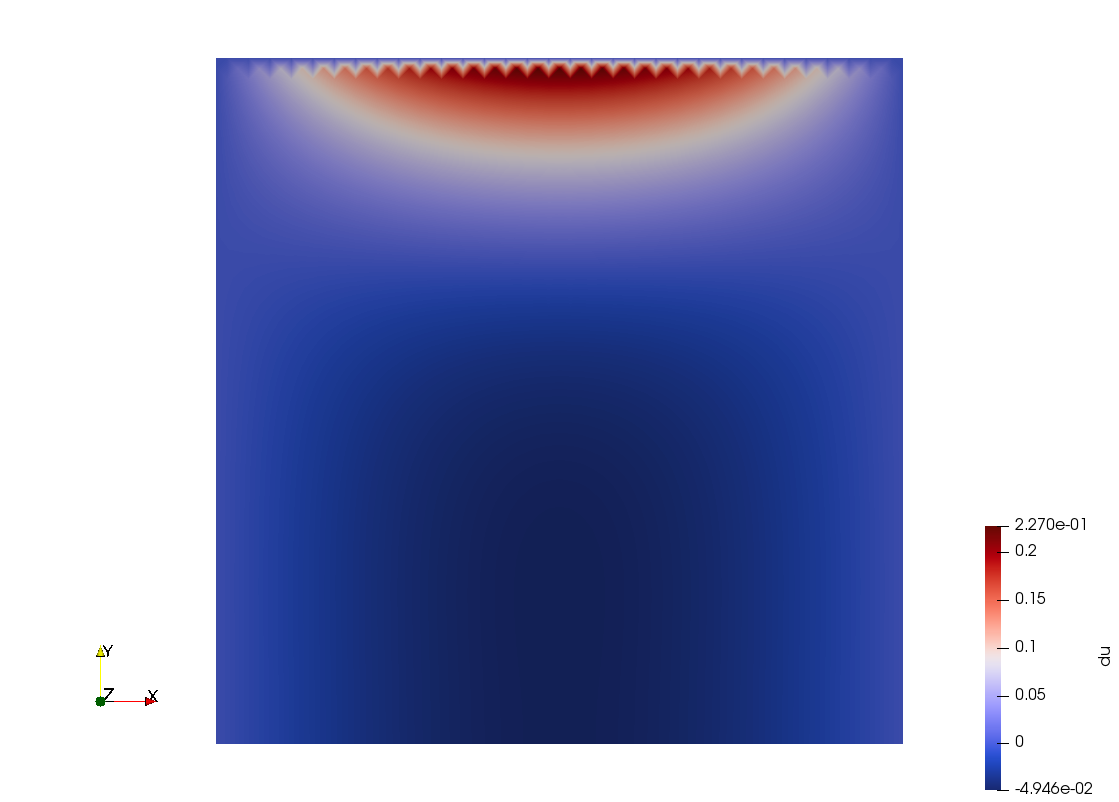
\includegraphics[width=4cm]{python_codes/fieldstone_87/results/experiment_00/du_00}
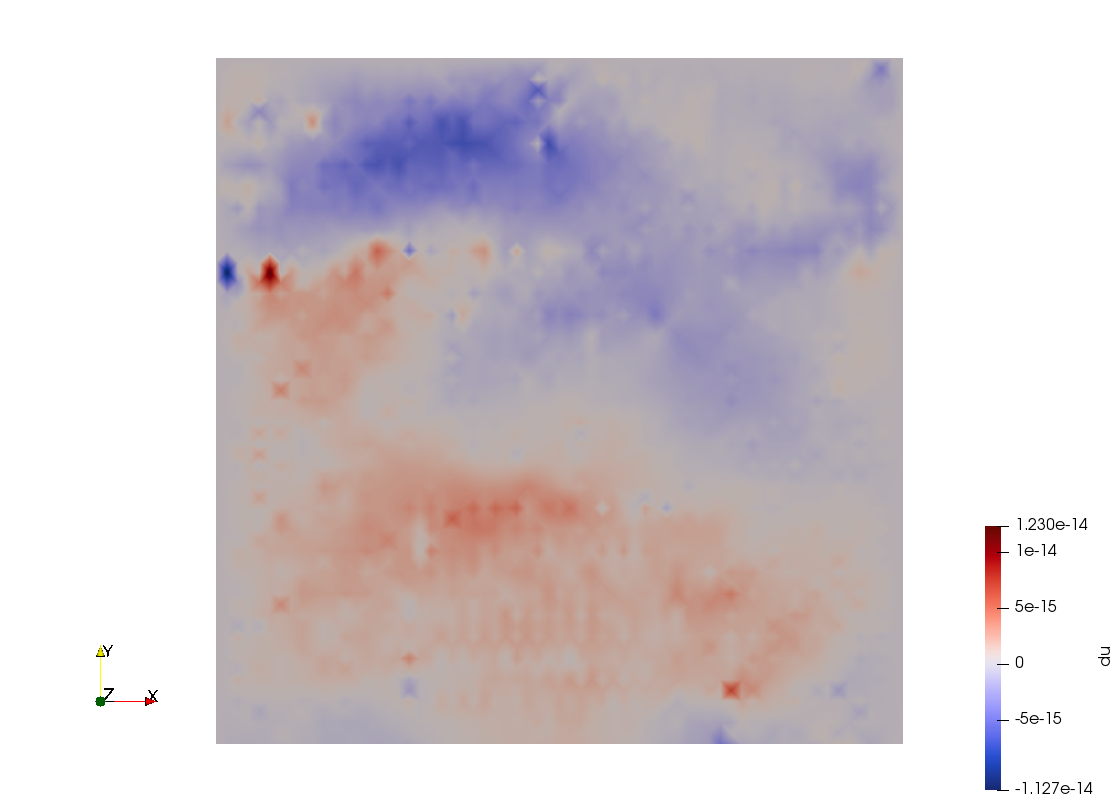
\includegraphics[width=4cm]{python_codes/fieldstone_87/results/experiment_00/du_01}
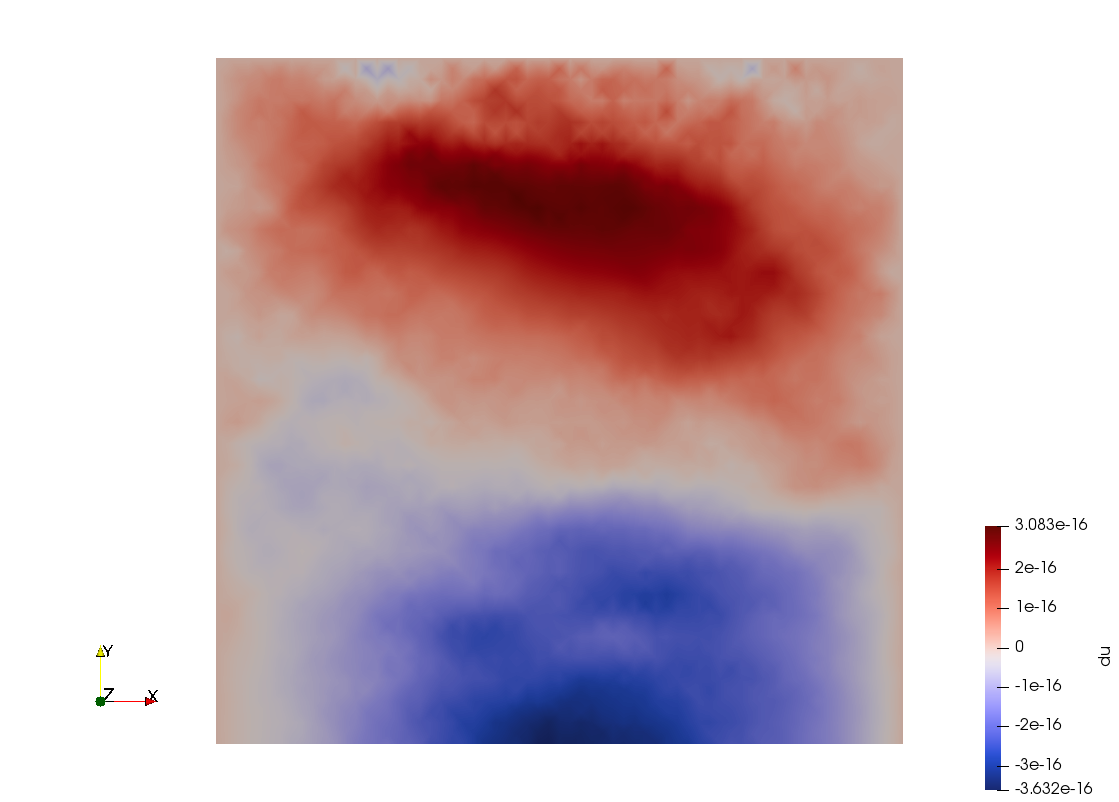
\includegraphics[width=4cm]{python_codes/fieldstone_87/results/experiment_00/du_02}
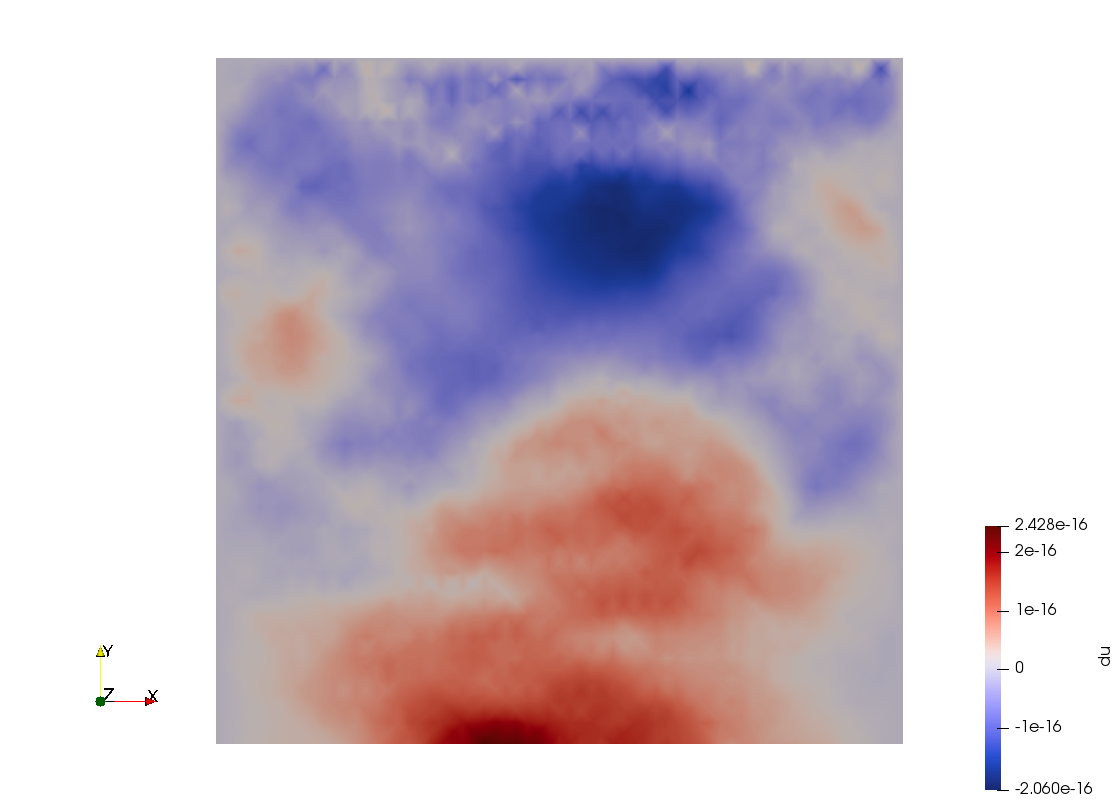
\includegraphics[width=4cm]{python_codes/fieldstone_87/results/experiment_00/du_03}\\
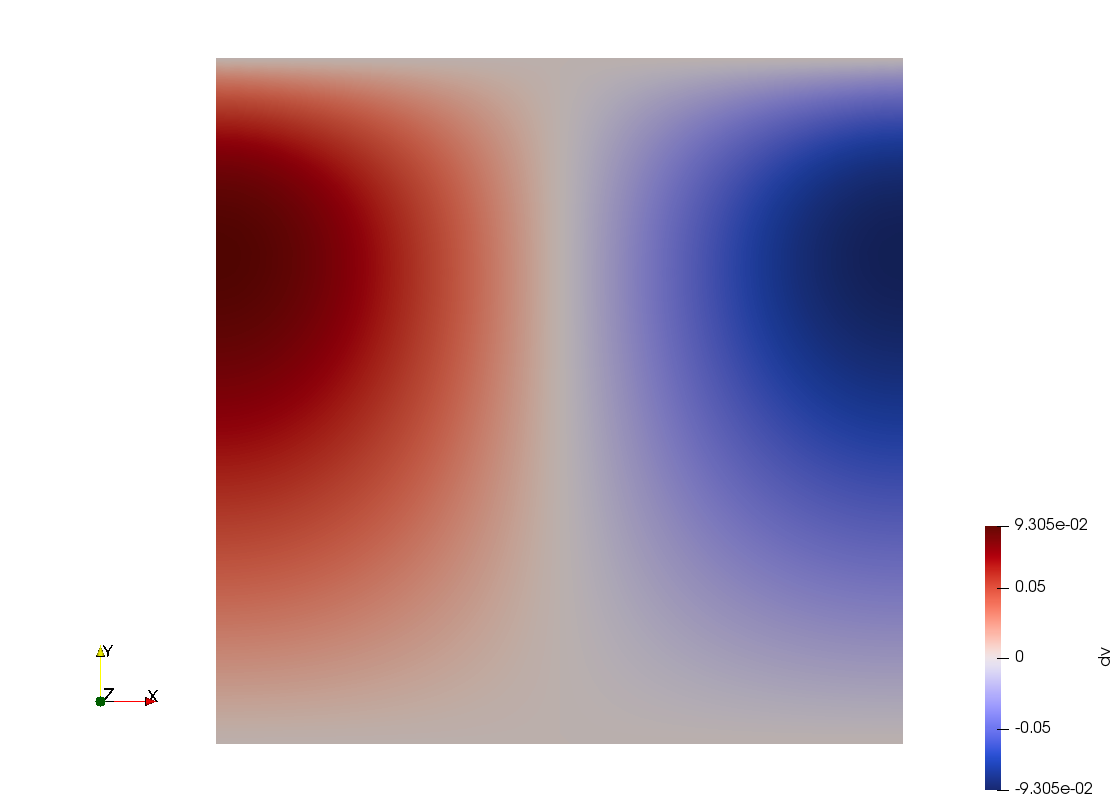
\includegraphics[width=4cm]{python_codes/fieldstone_87/results/experiment_00/dv_00}
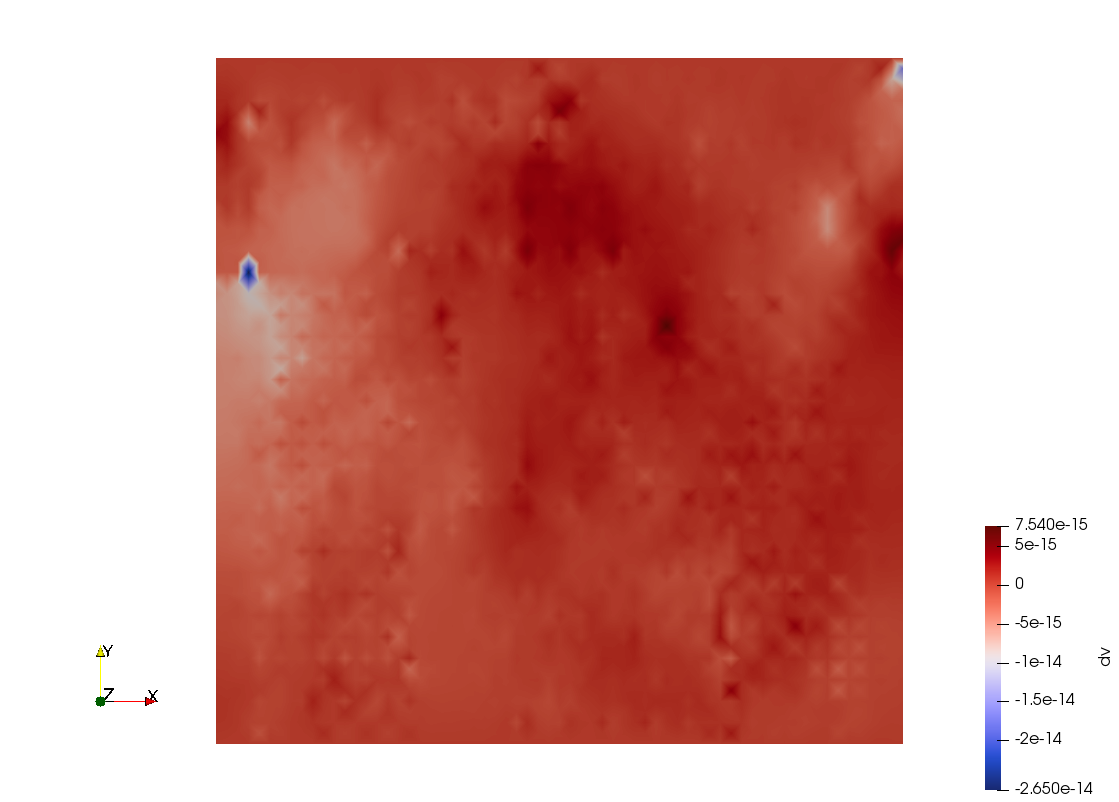
\includegraphics[width=4cm]{python_codes/fieldstone_87/results/experiment_00/dv_01}
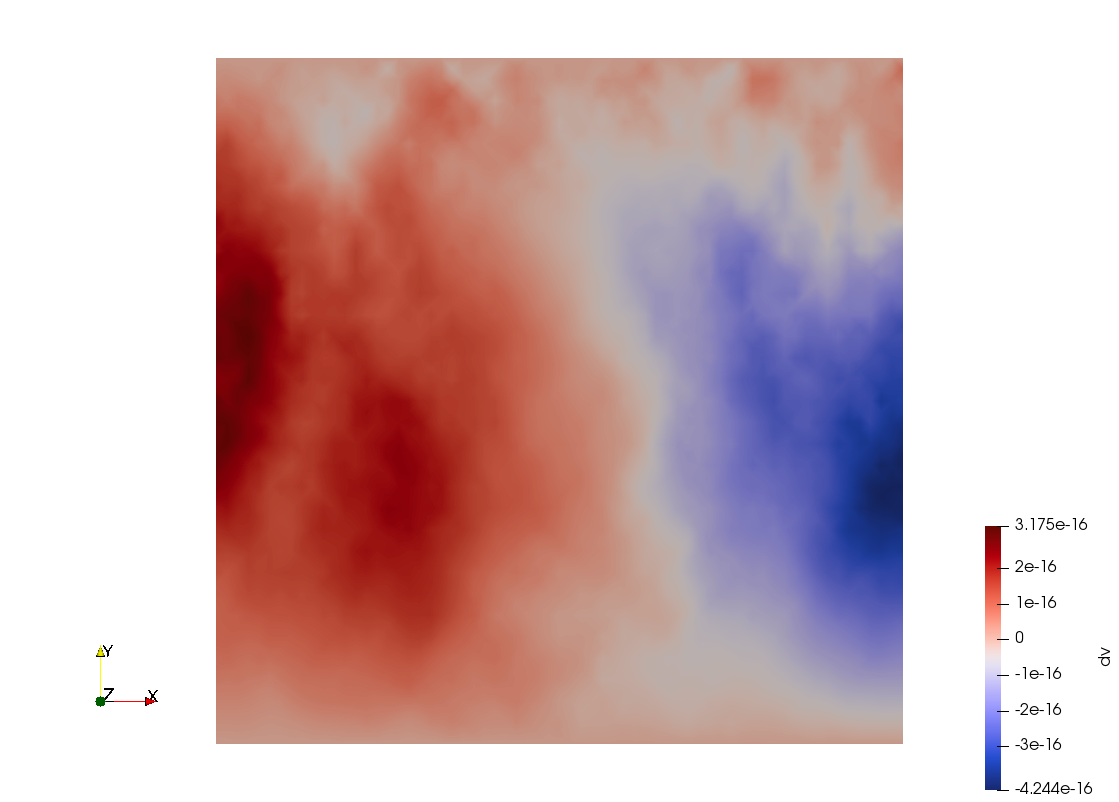
\includegraphics[width=4cm]{python_codes/fieldstone_87/results/experiment_00/dv_02}
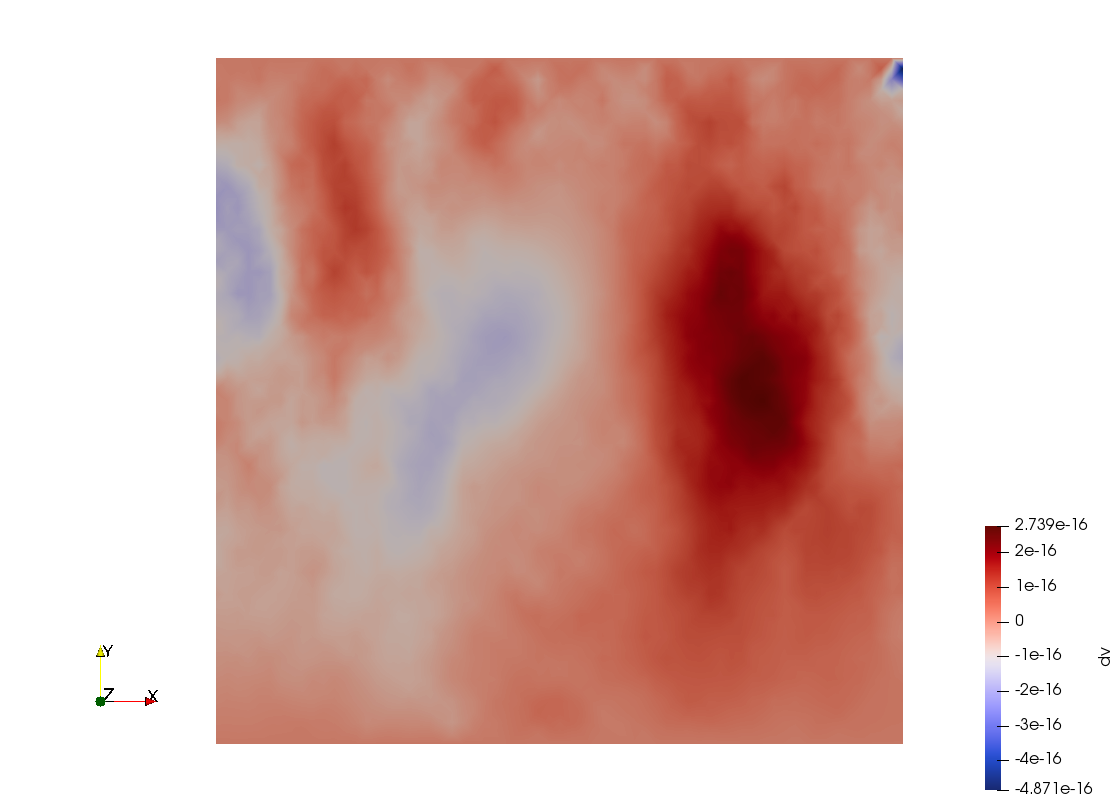
\includegraphics[width=4cm]{python_codes/fieldstone_87/results/experiment_00/dv_03}\\
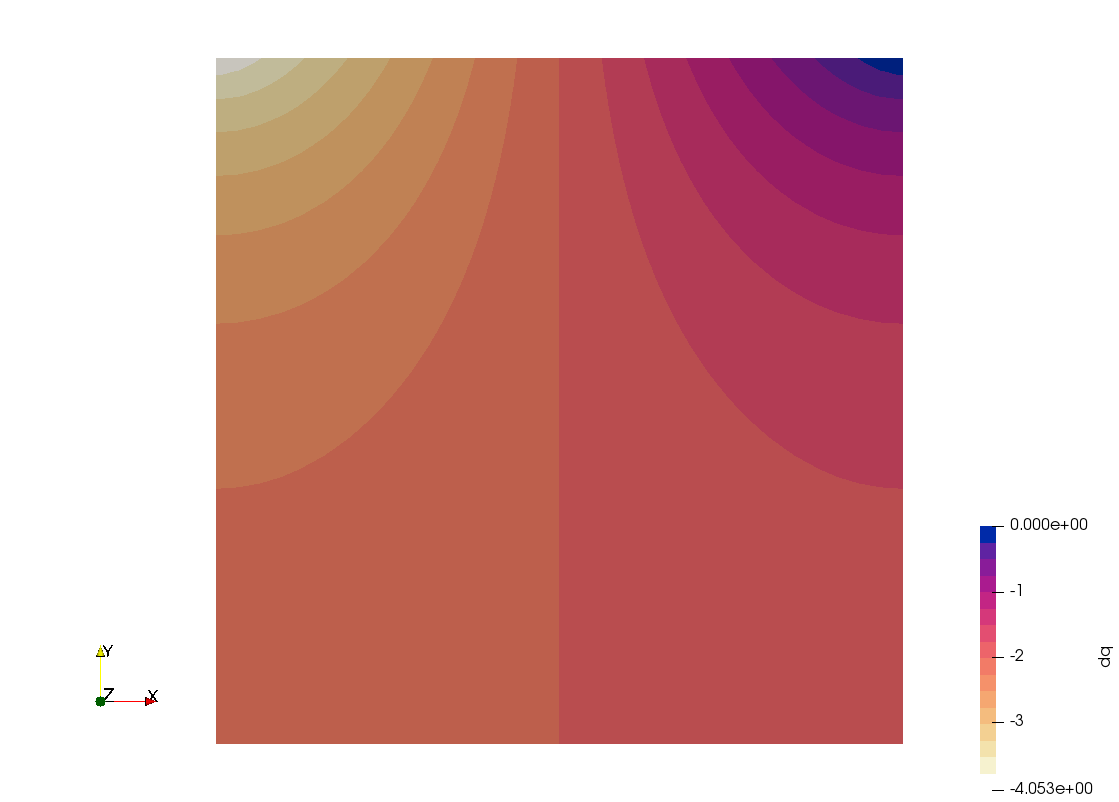
\includegraphics[width=4cm]{python_codes/fieldstone_87/results/experiment_00/dp_00}
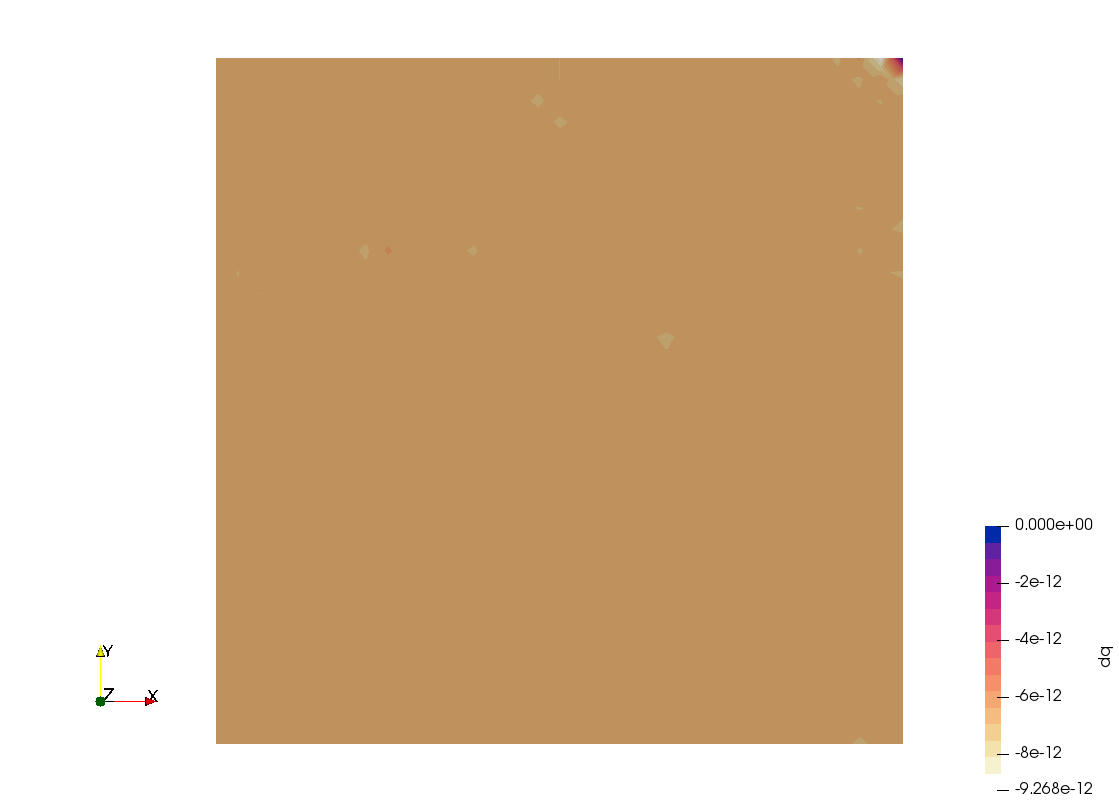
\includegraphics[width=4cm]{python_codes/fieldstone_87/results/experiment_00/dp_01}
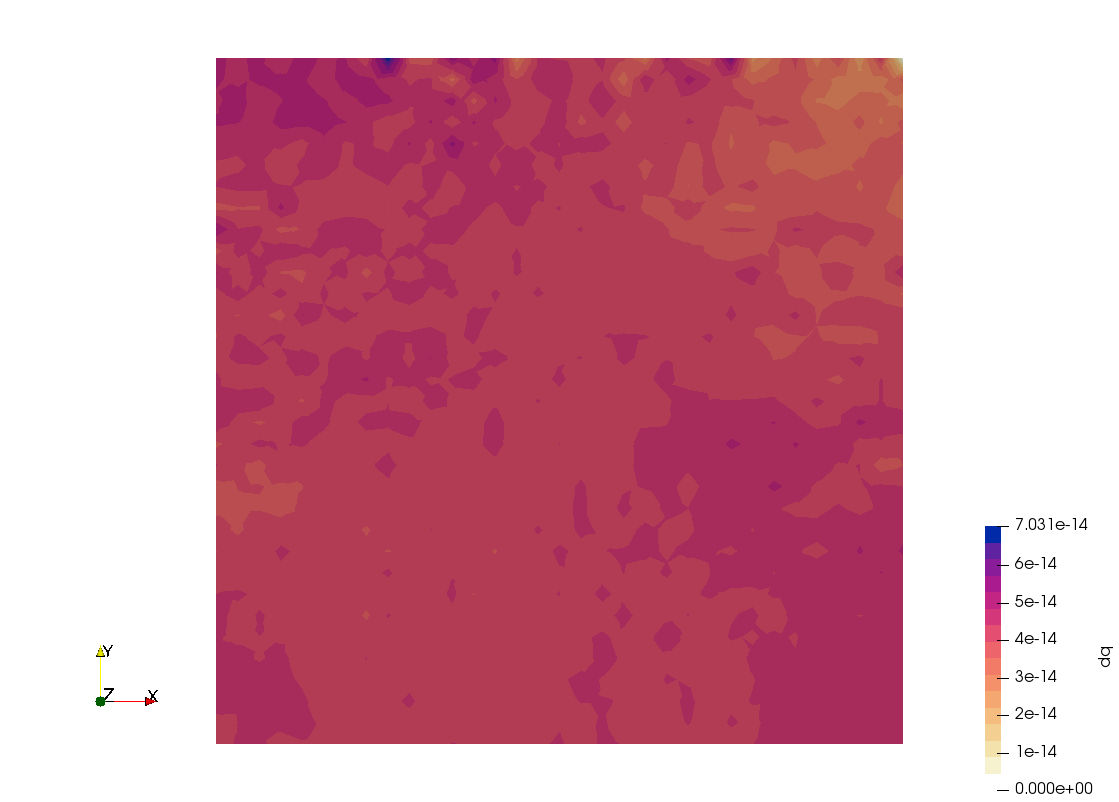
\includegraphics[width=4cm]{python_codes/fieldstone_87/results/experiment_00/dp_02}
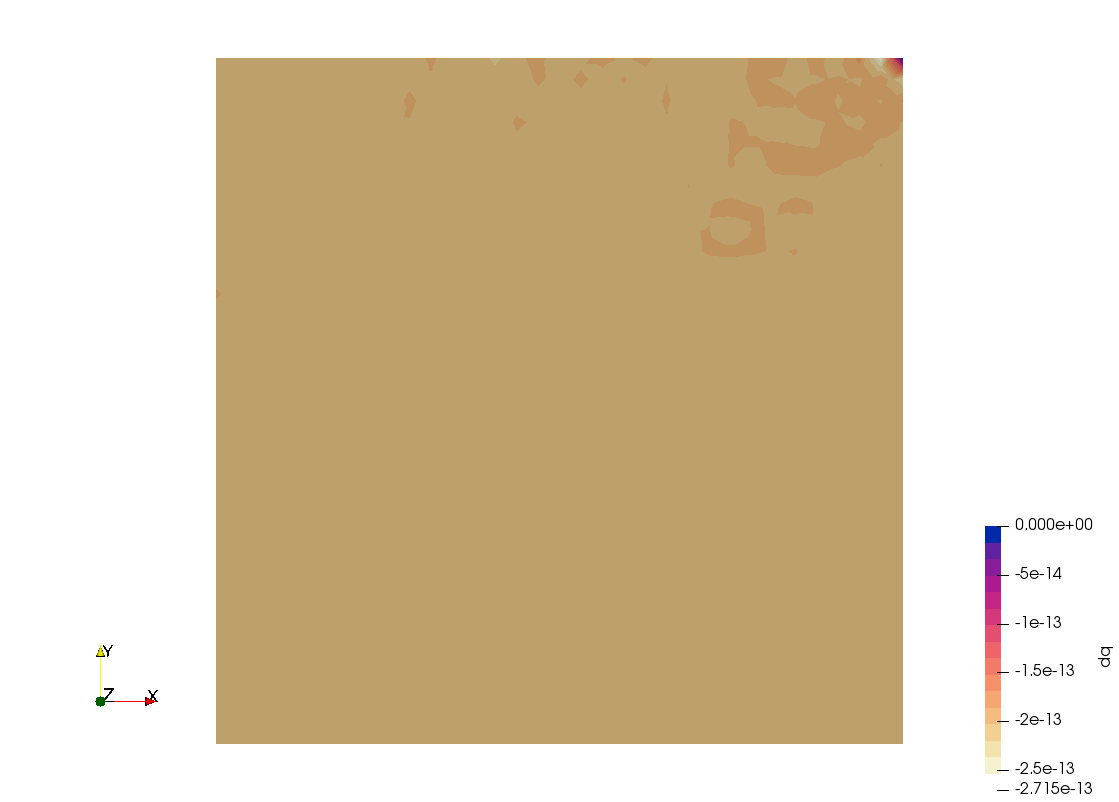
\includegraphics[width=4cm]{python_codes/fieldstone_87/results/experiment_00/dp_03}\\
{\captionfont From left to right: iteration 0,1,2,3. 
Top to bottom: horizontal component of the velocity correction, 
vertical component of the velocity correction, and pressure correction, 
as obtained on a $32\times 32$ grid. The fields obtained at iteration 0 
are in fact the solution, and all other subsequently obtained fields 
are essentially zero, as expected.}
\end{center}

%--------------------------------------------------------------------------
\subsubsection*{Experiment 1 - the (regularised) lid driven cavity}

This is the same experiment as above but the viscosity is now of the 
power law type with $\beta=1$ and $n>1$. 

reg param ?

\begin{center}
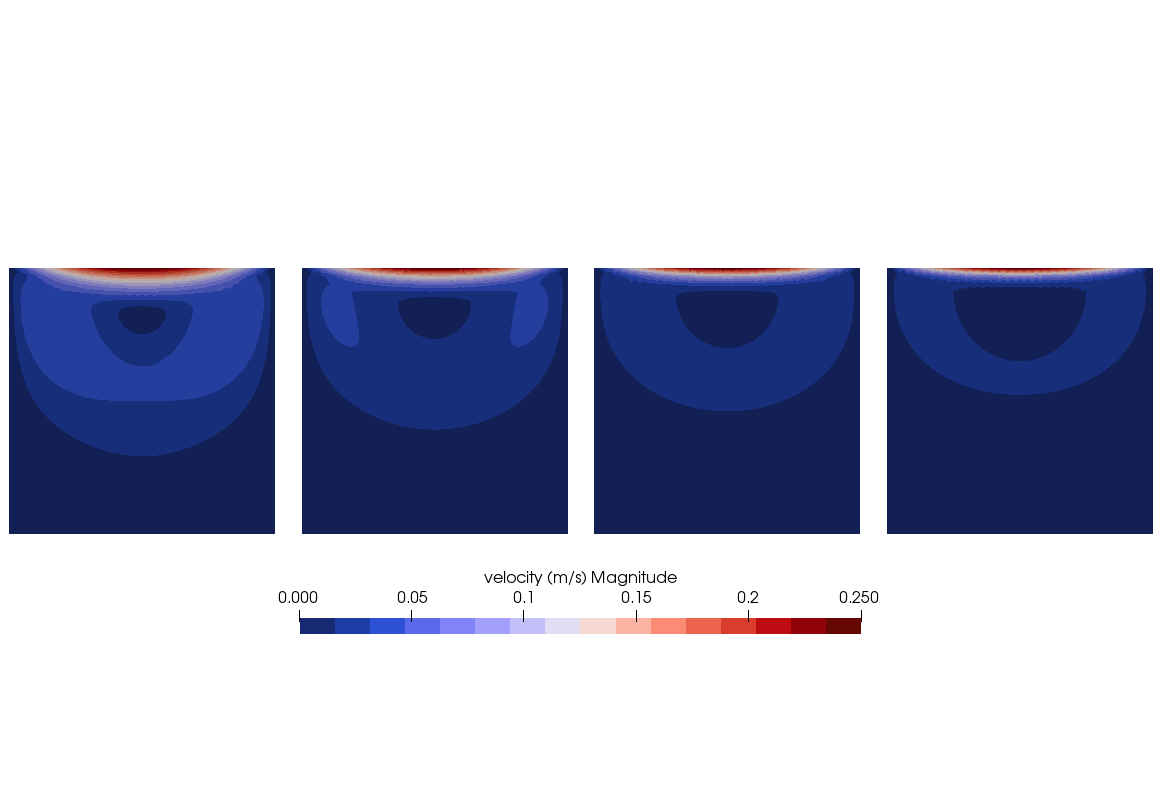
\includegraphics[width=7cm]{python_codes/fieldstone_87/results/experiment_01/vel.png}
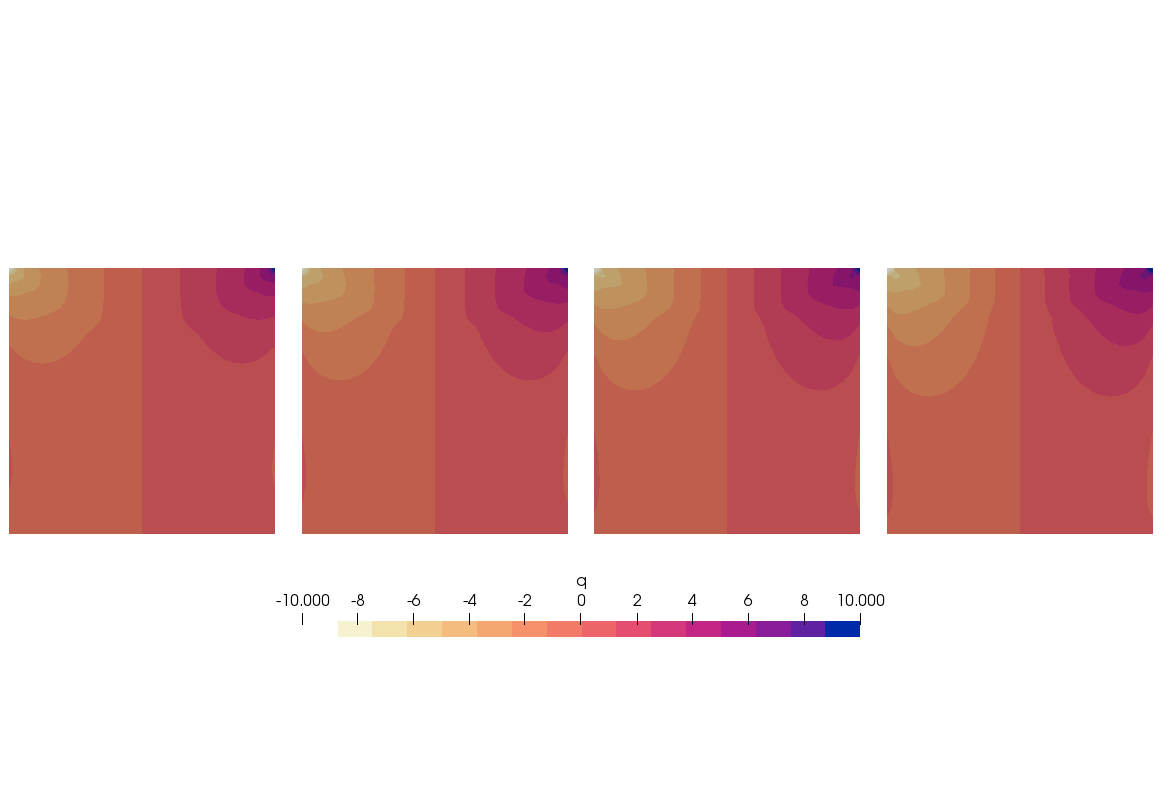
\includegraphics[width=7cm]{python_codes/fieldstone_87/results/experiment_01/p.png}\\
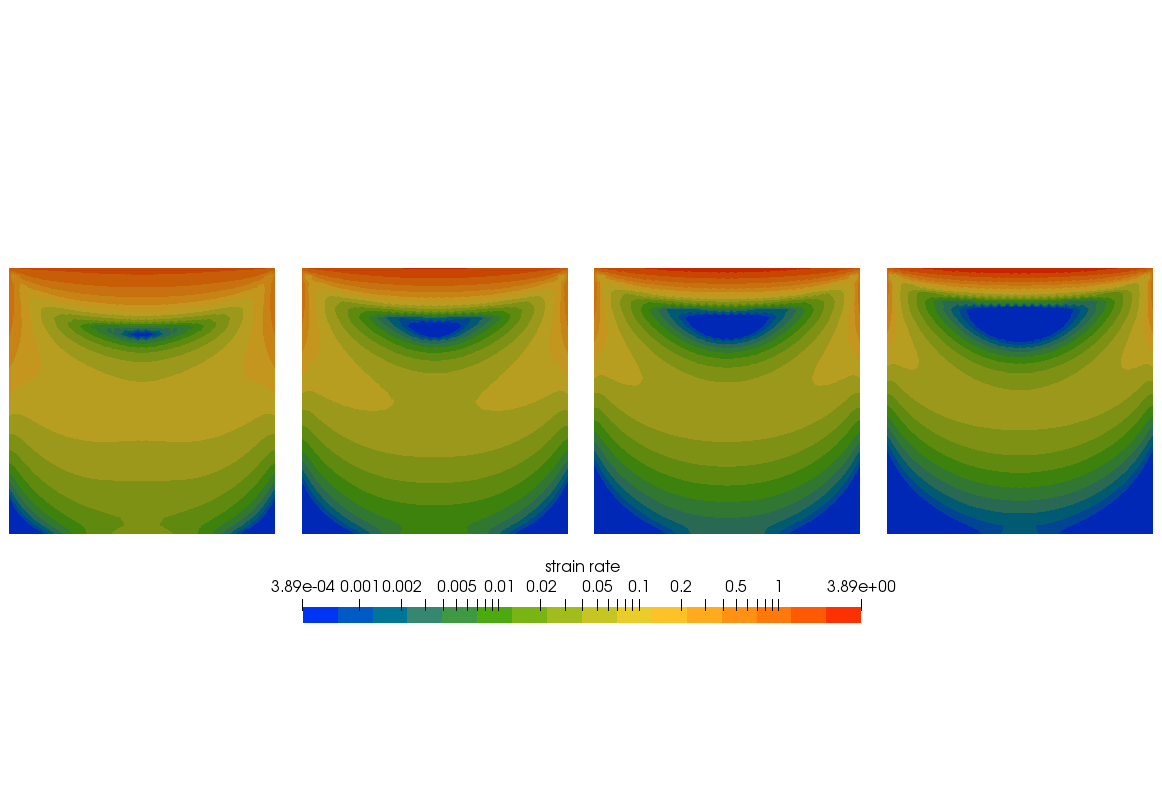
\includegraphics[width=7cm]{python_codes/fieldstone_87/results/experiment_01/sr.png}
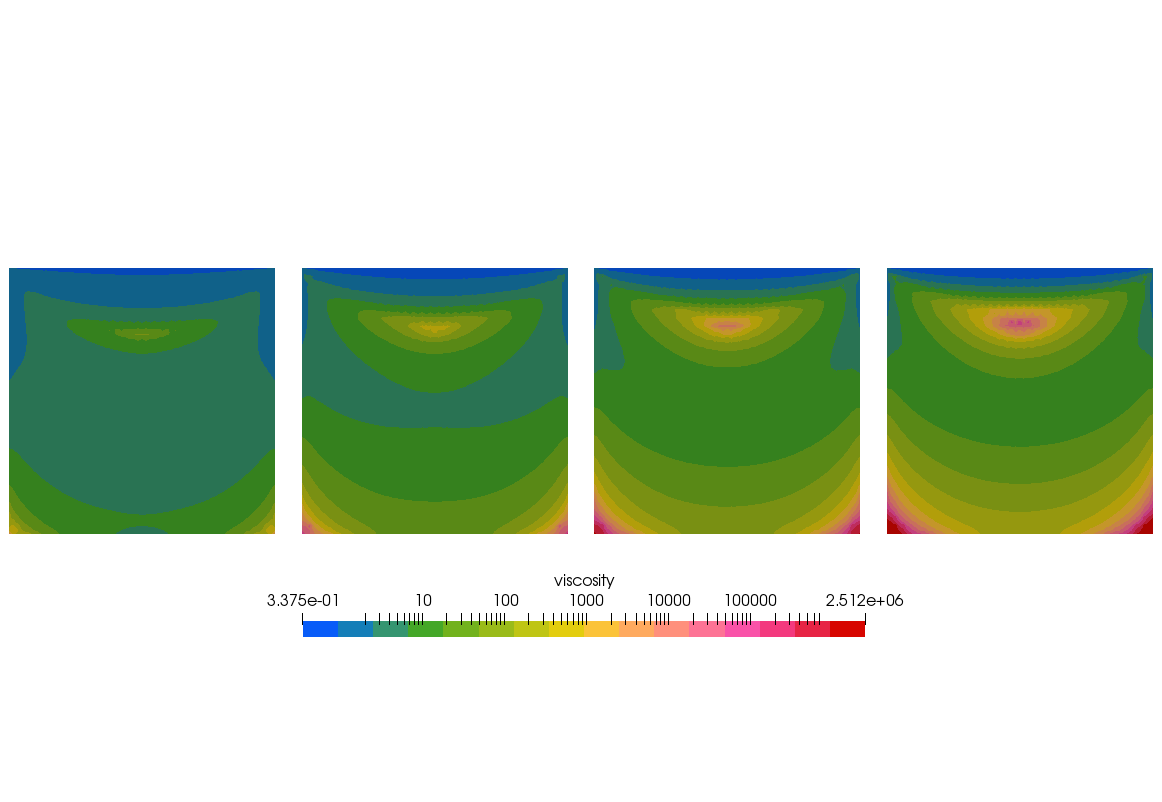
\includegraphics[width=7cm]{python_codes/fieldstone_87/results/experiment_01/eta.png}
\end{center}


\begin{center}
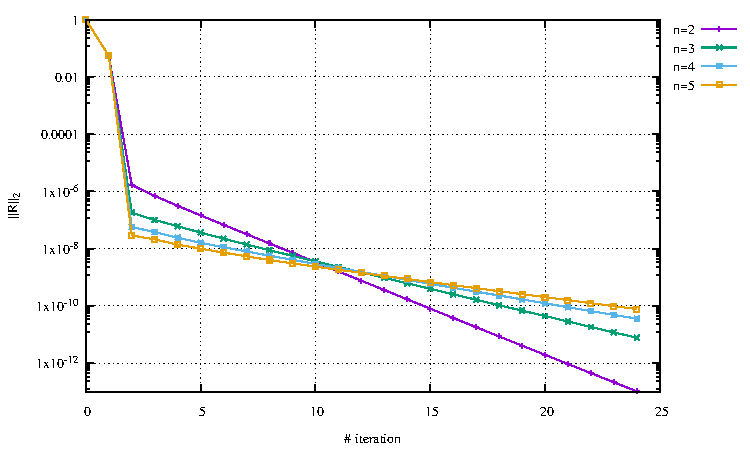
\includegraphics[width=5.7cm]{python_codes/fieldstone_87/results/experiment_01/conv}
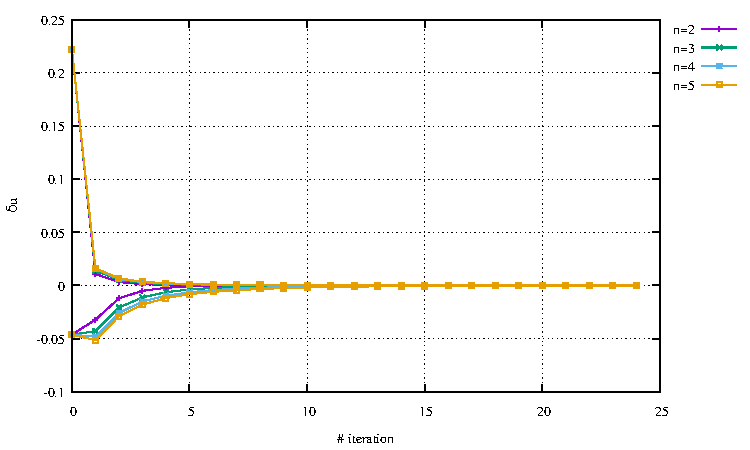
\includegraphics[width=5.7cm]{python_codes/fieldstone_87/results/experiment_01/du}
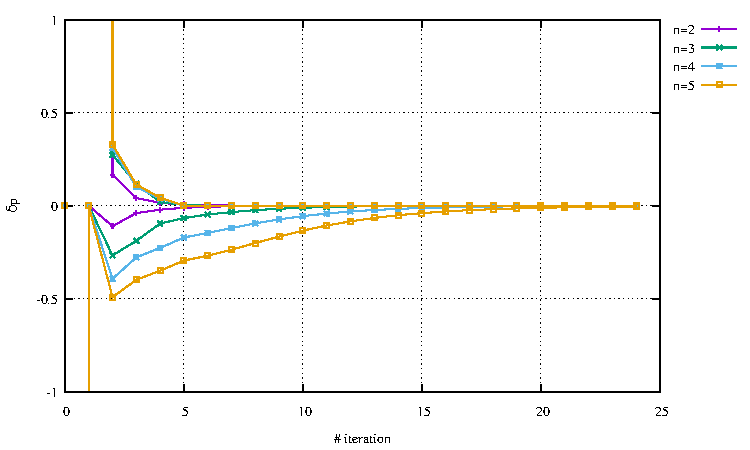
\includegraphics[width=5.7cm]{python_codes/fieldstone_87/results/experiment_01/dp}\\
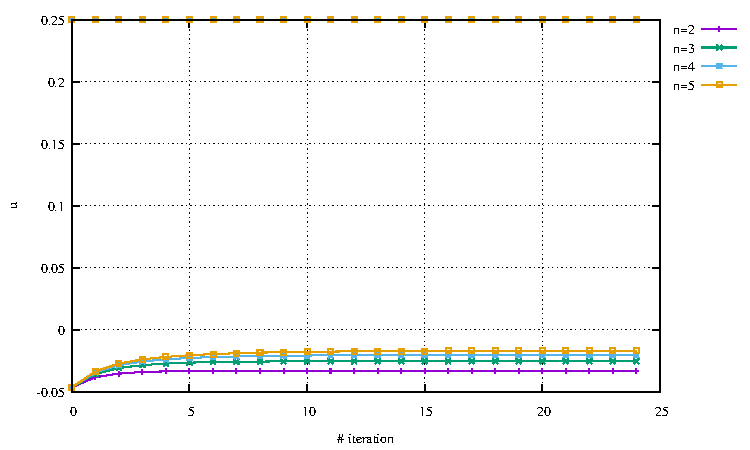
\includegraphics[width=5.7cm]{python_codes/fieldstone_87/results/experiment_01/u}
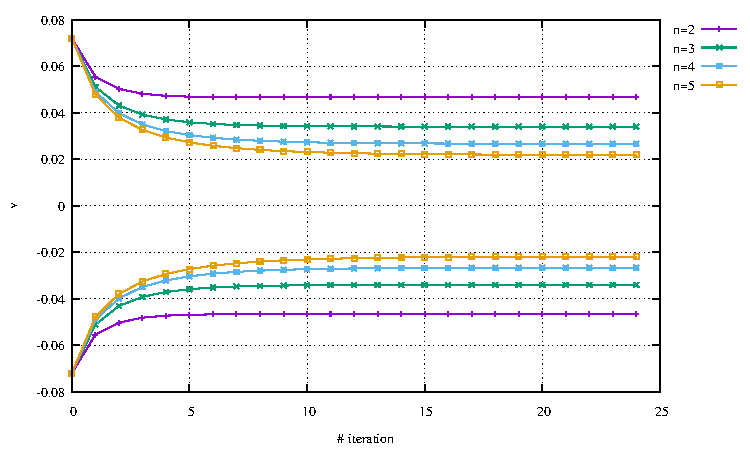
\includegraphics[width=5.7cm]{python_codes/fieldstone_87/results/experiment_01/v}
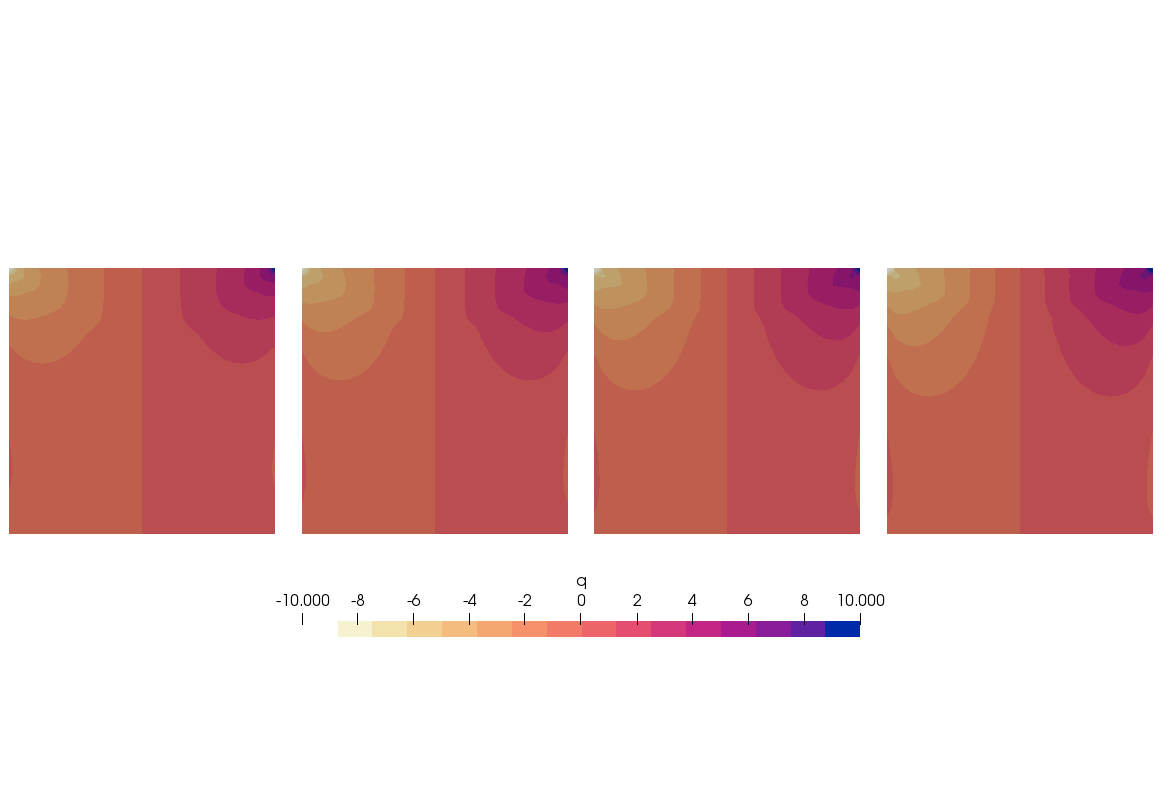
\includegraphics[width=5.7cm]{python_codes/fieldstone_87/results/experiment_01/p}
\end{center}





